\def\layersep{1.5cm}

\def\checkmark{\tikz\fill[scale=0.8, color=green_jon](0,.35) -- (.25,0) -- (1,.7) -- (.25,.15) -- cycle;} 
\definecolor{green_jon}{rgb}{0.0, 0.5, 0.0}

\begin{frame}{Geophysics Synthetic Example: Input Measurements}
\vspace{-0.35 cm}
\begin{figure}[H]
	\centering
	\begin{tikzpicture}[scale=1.0]
	\node (layers) at (0.0,0.0)[scale=0.7]{
		\begin{tikzpicture}

%% Tool
\fill[gray!80!white] (-1.5*3,0) -- (1.5*3,0.) --  node[right] {\small \bf \textcolor{black}{500 kHz}}  (1.5*3, 0.15*3) -- (-1.5*3,0.15*3) -- cycle;

%% Transmitters
\fill[black!80!white] (-0.6096*5-0.02*3,0) -- (-0.6096*5+0.02*3,0.) -- (-0.6096*5+0.02*3, 0.15*3) node[above] {\footnotesize \bf \textcolor{black}{Tx$_1$}}  -- (-0.6096*5-0.02*3,0.15*3) -- cycle;
%
\fill[black!80!white] (0.6096*5-0.02*3,0) -- (0.6096*5+0.02*3,0.)  -- (0.6096*5+0.02*3, 0.15*3) node[above] {\footnotesize \bf \textcolor{black}{Tx$_2$}} -- (0.6096*5-0.02*3,0.15*3) -- cycle;

%% Receivers
\fill[red!80!white] (-0.1016*5-0.02*3,0) -- (-0.1016*5+0.02*3,0.)  -- (-0.1016*5+0.02*3, 0.15*3) node[above] {\footnotesize \bf \textcolor{black}{Rx$_1$}} -- (-0.1016*5-0.02*3,0.15*3) -- cycle;
\fill[red!80!white] ( 0.1016*5-0.02*3,0) -- ( 0.1016*5+0.02*3,0.) -- ( 0.1016*5+0.02*3, 0.15*3)  node[above] {\footnotesize \bf \textcolor{black}{Rx$_2$}} -- ( 0.1016*5-0.02*3,0.15*3) -- cycle;

%% distances
\draw[black, line width=1pt,<->] (-0.1016*5, -0.6)      -- (0.1016*5, -0.6) node[pos=0.5, below] {\footnotesize \bf \textcolor{black}{0.40 m}}  ;
\draw[gray, dashed] (-0.1016*5, -0.6)      -- (-0.1016*5, 0)  ;
\draw[gray, dashed] ( 0.1016*5, -0.6)      -- ( 0.1016*5, 0)  ;

\draw[black, line width=1pt,<->] (-0.6096*5, -1.2)      -- (0.6096*5, -1.2) node[pos=0.5, below] {\footnotesize \bf \textcolor{black}{1.8 m}}  ;
\draw[gray, dashed] (-0.6096*5,-1.2)      -- (-0.6096*5, 0)  ;
\draw[gray, dashed] ( 0.6096*5,-1.2)      -- ( 0.6096*5, 0)  ;


\end{tikzpicture}
	};       
	\end{tikzpicture}
\end{figure}
\vspace{-0.7 cm}

	\begin{itemize}
		\item Co-axial attenuation and phase difference
	\end{itemize}
	
	\vspace{0.4 cm}

\begin{figure}[H]
	\centering
	\begin{tikzpicture}[scale=1.0]
	\node (layers) at (0.0,0.0)[scale=0.7]{
		\input{Diapos/DL_For_Inv/Figures/Syn_example/Fig_tool2.tex}
	};       
	\end{tikzpicture}
\end{figure}
\vspace{-0.7 cm}
	\begin{itemize}
		\item Co-axial attenuation and phase difference
		\item Geosignal
	\end{itemize}
\end{frame}


\begin{frame}{Geophysics Synthetic Example: Output Earth Parametrization}
\begin{columns}
    \begin{column}{0.35\textwidth}
    \begin{figure}[!h]
	\centering
	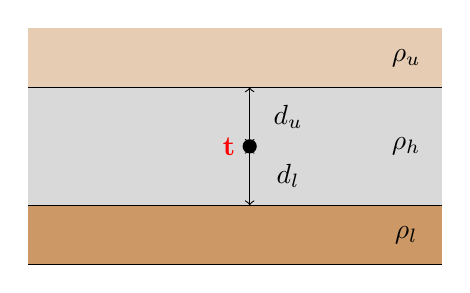
\begin{tikzpicture}[scale=1.5]
\draw (0,0) rectangle (3.5,2);

\fill[white!20!brown] (0,0) rectangle (3.5,0.5);
\fill[white!70!gray] (0,0.5) rectangle (3.5,1.5);
\fill[white!60!brown] (0,1.5) rectangle (3.5,2);


%\draw[red, line width=0.5 mm] (0.75,1.5) .. controls (1.15,1.1) .. (1.85,1) node (n1) at (0.85,1.6) {$\mathbf{t}$};
\draw[black, line width=0.1 mm] (0,0.5) -- (3.5,0.5);
\draw[black, line width=0.1 mm] (0,1.5) -- (3.5,1.5);

\fill[black] (1.875,1) circle (0.06cm);
\node (d_u) at (1.7,1) {\textcolor{red}{$\textbf{t}$}};
\draw[<->] (1.875,1.02) -- (1.875,1.5);
\node (d_u) at (2.2,1.25) {$d_u$}; 
\draw[<->] (1.875,0.98) -- (1.875,.5);
\node (d_u) at (2.2,0.75) {$d_l$};
\node (rho) at (3.2,1.75) {$\rho_u$};
\node (rho) at (3.2,0.25) {$\rho_l$};
\node (rho) at (3.2,1) {$\rho_h$};
\end{tikzpicture}

	\label{fig:param}
	\end{figure}
    \end{column}
    \begin{column}{0.5\textwidth}
        {\footnotesize $\rho_u \in [1,10^2] \Omega \cdot m$: Upper layer resistivity}\\
        \vspace{0.3cm}
        {\footnotesize $\rho_h \in [1,10^2] \Omega \cdot m$: Central layer resistivity}\\
        \vspace{0.3cm}
        {\footnotesize $\rho_l \in [1,10^2] \Omega \cdot m$: Lower layer resistivity}\\
        \vspace{0.3cm}
        {\footnotesize $d_u \in [10^{-2},10] m$: Vertical distance to upper layer}\\
        \vspace{0.3cm}
        {\footnotesize $d_l \in [10^{-2},10] m$: Vertical distance to lower layer}
    \end{column}
\end{columns}
\end{frame}


%\begin{frame}[t]{Deep Neural Networks (Deep Learning) for Inverse Problems}\linespread{1.05}
%\vspace{-.2 cm}
%\begin{center}
%	Approximate: ${\cal I} \approx {\cal I}_{\phi} :=  N \circ A_k \circ N \circ A_{k-1}  \circ \cdots \circ N \circ A_1 $\\
%\end{center}
%\only<1>{
%	\vspace{0.2 cm}
%	\centerline{$N$ -- Non-linear activation function  \hspace{0.3 cm};\hspace{0.3 cm} $A_k$ -- Affine transformation}
%	\vspace{0.6cm}
%\begin{figure}
%	\vspace*{-0.25in}
%	\begin{tikzpicture}
	\visible<2>{
	\node[] () at (0,-0.2) {\begin{tikzpicture}[scale=0.62]
		\begin{axis}[
		%ticks=none,
		height=0.5\textwidth,
		width=0.1\textwidth,
		scale only axis,
		enlargelimits=false,
		axis on top,
		xlabel={Resistivity [$\Omega$m]},
		xtick={0,1.2,2.39},
		xticklabels={100,200,300},
		ytick={0.93,1.85,2.78,3.7,4.65,5.56,6.50,7.44,8.37,9.305,10.24,11.18,12.08,13},
		yticklabels={130,120,110,100,90,80,70,60,50,40,30,20,10,0},
		ylabel={Deep [m]},
		label style={font=\tiny},
		tick label style={font=\tiny}] 
		\addplot[thick] graphics[xmin=0,xmax=3,ymin=0,ymax=13] {Diapos/Intro/Figures/resis1};
		\end{axis}
		\end{tikzpicture}};
		}
		
	\node[] () at (4.3,0.2) {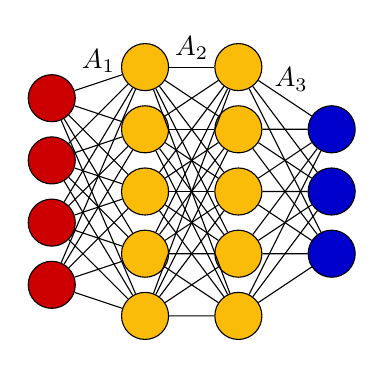
\begin{tikzpicture}[scale=0.79]
		\tikzstyle{every pin edge}=[<-,shorten <=1pt]
		\tikzstyle{neuron}=[circle,fill=black!25,minimum size=17pt,inner sep=0pt]
		\tikzstyle{input neuron}=[neuron,draw=black,fill=red!80!black];
		\tikzstyle{output neuron}=[neuron,draw=black,fill=blue!80!black];
		\tikzstyle{hidden neuron}=[neuron,draw=black,fill=yellow!50!orange];
		\tikzstyle{annot} = [text width=4em, text centered]
			
			% Draw the input layer nodes
		\foreach \name / \y in {1,...,4}
		% This is the same as writing \foreach \name / \y in {1/1,2/2,3/3,4/4}
		\node[input neuron] (I-\name) at (0,-\y) {};
			
			% Draw the hidden layer nodes
		\foreach \name / \y in {1,...,5}
		\path[yshift=0.5cm]
		node[hidden neuron] (H-\name) at (\layersep,-\y cm) {};
			
			% Draw the hidden layer nodes
		\foreach \name / \y in {1,...,5}
		\path[yshift=0.5cm]
		node[hidden neuron] (H2-\name) at (\layersep+\layersep,-\y cm) {};
			
			
			% Draw the output layer node
		\foreach \name / \y in {1,...,3}
		\path[yshift=-0.5cm]
		node[output neuron] (O-\name) at (\layersep+\layersep+\layersep,-\y cm) {};
			
			% Connect every node in the input layer with every node in the
			% hidden layer.
		\foreach \source in {1,...,4}
		\foreach \dest in {1,...,5}
		\path (I-\source) edge (H-\dest);
			
		\foreach \source in {1,...,5}
		\foreach \dest in {1,...,5}
		\path (H-\source) edge (H2-\dest);
			
			% Connect every node in the hidden layer with the output layer
		\foreach \source in {1,...,5}
		\foreach \dest in {1,...,3}
		\path (H2-\source) edge (O-\dest);

	    \node[] () at (0.75, -.4) {$A_1$};	
		\node[] () at (2.25, -0.2) {$A_2$};
		\node[] () at (3.85,-.7) {$A_3$};
			% Annotate the layers
		\end{tikzpicture}};
	\node[] () at (4.3, 2.8) {Neural Network};		
	\visible<2>{	
	\node[] () at (8.8, 1.2) {\includegraphics[width=2.5cm]{Diapos/Intro/Figures/res1}};
	\node[] () at (8.8,-1.4) {\includegraphics[width=2.5cm]{Diapos/Intro/Figures/res2}};
	\node[] () at (8.4, 2.8) {Output};
	\node[] () at (0.2, 2.8) {Input};
		
	\draw [decorate,very thick,decoration={brace,amplitude=10pt},xshift=-4pt,yshift=0pt]
		(1.3,2.8) -- (1.3,-2.4);
	\draw [decorate,very thick,decoration={brace,amplitude=10pt},xshift=-4pt,yshift=0pt]
		(7.5,-2.4) -- (7.5,2.8);
		
	\node[right] () at (9.0, 0.0) {\scriptsize Water};		
	\node[right] () at (9.0, -2.5) {\scriptsize Oil};	
	}			
\end{tikzpicture}
%\end{figure}}
%\only<2>{
%	\vspace{0.4cm}
%	
%	$A_k$ -- Affine transformation: \hspace{0.1cm} $A_k \cdot x+b_k$
%	\vspace{0.4cm}
%	
%	$N$ -- Non-linear activation function:
%
%	\begin{figure}
%	\centering
%		\begin{subfigure}{.5\textwidth}
%		\centering
%		\begin{tikzpicture}[scale=0.7]
\begin{axis}[
    xmin=-2.5, xmax=2.5,
    ymin=-1.5, ymax=1.5,
    axis lines=center,
    axis on top=true,
    domain=-2.5:2.5,
    ylabel=$tanh(x)$,
    xlabel=$x$,
    x label style={at={(axis description cs:0.5,-0.1)},anchor=north},
    y label style={at={(axis description cs:-0.1,.5)},rotate=90,anchor=south},
    ]

    \addplot [mark=none,draw=blue,ultra thick] {tanh(\x)};
%    \node [right, red] at (axis cs: 1,0.7) {$y = \tanh x$};
    
    %% Add the asymptotes
%    \draw [blue, dotted, thick] (axis cs:-2.5,-1)-- (axis cs:0,-1);
%    \draw [blue, dotted, thick] (axis cs:+2.5,+1)-- (axis cs:0,+1);
\end{axis}
\end{tikzpicture}

%		%	\caption{Tanh}
%		\label{fig:tanh}
%		\end{subfigure}%
%		\begin{subfigure}{.5\textwidth}
%		\centering
%		\begin{tikzpicture}[scale=0.7,
  declare function={
    func(\x)= (\x < 0) * (0)   +
                   + (\x >= 0) * (\x);
  }
]
\begin{axis}[
    xmin=-2.5, xmax=2.5,
    ymin=-1.5, ymax=1.5,
    axis lines=center,
    axis on top=true,
    domain=-2.5:2.5,
  ylabel=$ReLU(x)$,
  xlabel=$x$,
     x label style={at={(axis description cs:0.5,-0.1)},anchor=north},
    y label style={at={(axis description cs:-0.1,.5)},rotate=90,anchor=south}, % added
]

\addplot [blue,ultra thick] {func(x)};
\end{axis}
\end{tikzpicture} 
%		%	\caption{Tanh}
%		\label{fig:tanh}
%		\end{subfigure}
%%	\caption{A figure with two subfigures}
%	\label{fig:test}
%	\end{figure}
%	}
%\end{frame}


\begin{frame}{Synthetic Example}
\begin{center}
{\large Formation of model problem}
\end{center}
\begin{figure}
		\centering
		\input{Diapos/DL_For_Inv/Figures/Syn_example/Numerical_results/real.tex}
	%\caption{Formation of model problem}
	\label{fig:formation_model_1_original}
\end{figure}
\end{frame}


\begin{frame}{Encoder-Decoder Loss}
\begin{center}
{\large Predicted formation}
\end{center}
\begin{figure}
		\centering
		\pgfplotsset{every axis legend/.append style={
		at={(0.5,1.03)},
		anchor=south},
	every axis plot/.append style={line width=1.8pt},
}
\begin{tikzpicture}
\begin{axis}[
%  ymode=log,
%  xmode=log,
%  grid=both,
%xmin=0,
%xmax=540,
legend columns=2,
%  ymin=-20.0,
%  ymax=-11,
height=0.25*\textwidth,
width=0.7*\textwidth,
% 
 y dir=reverse,
xlabel={HD ($m$)},
ylabel near ticks,
ylabel={TVD ($m$)},
%axis equal image,
enlargelimits=false,
]

%[enlargelimits=false, axis on top, axis equal image, width=6cm]

%\node[] at (rel axis cs:0,0) {\includegraphics{Syn_1/Predicted.png}};

\addplot graphics[xmin=0,xmax=540,ymin=45,ymax=60] {frames/JonAnder/Latex_files/Figures/Enco-Deco/Predicted_F_FI.png};

\end{axis}	
\end{tikzpicture}

	%\caption{Formation of model problem}
	\label{fig:formation_model_1_original}
\end{figure}
\end{frame}


\begin{frame}{Cross-plot 1}
\centering
\setlength{\fboxrule}{0.5mm}
\setlength{\fboxsep}{1mm}
\color{red}
\fbox{\parbox{3cm}{{\begin{align}
\textcolor{black}{\mathcal{F} \circ \mathcal{I} \hspace{0.25cm} vs \hspace{0.25cm} \mathcal{F}_{\theta^\ast} \circ \mathcal{I}}
\notag
\end{align}}}}
\color{black}
To control: $\|{\cal F}_{\theta}({\bf P})-{\bf M} \|$ \hspace{1cm}  \visible<2>{\checkmark} \\
$\qquad$ \\
\hspace{0.8cm} Attenuation Geosignal $\qquad \qquad \qquad$ Phase difference Geosignal
\begin{figure}[!h]
\centering
	{\includegraphics[scale=0.9]{Diapos/DL_For_Inv/Figures/Syn_example/Cross_plots/C_P_1/Atten-Geosignal_axis.pdf}%}
		\hspace{2cm}
	\includegraphics[trim=0cm 0cm 0.3cm 0.25cm ,scale=0.9]{Diapos/DL_For_Inv/Figures/Syn_example/Cross_plots/C_P_1/Phase-Geosignal_axis.pdf}}	
\end{figure}
\end{frame}
%==========================================================
\begin{frame}{Cross-plot 2}
\centering
\setlength{\fboxrule}{0.5mm}
\setlength{\fboxsep}{1mm}
\color{red}
\fbox{\parbox{3cm}{{\begin{align}
\textcolor{black}
{\mathcal{F} \circ \mathcal{I} \hspace{0.25cm} vs \hspace{0.25cm} \mathcal{F}_{\theta^\ast} \circ \mathcal{I}_{\phi^\ast}}
\notag
\end{align}}}}
\color{black}
To control: $\|(\mathcal{F}_{\theta} \circ \mathcal{I}_{\phi})(\mathbf{M})-\mathbf{M}\|$ \hspace{1cm} \visible<2>{\checkmark} \\
$\qquad$ \\
\hspace{0.8cm} Attenuation Geosignal $\qquad \qquad \qquad$ Phase difference Geosignal
\begin{figure}[!h]
\centering
	{%
		\includegraphics[scale=0.9]{Diapos/DL_For_Inv/Figures/Syn_example/Cross_plots/C_P_2/Atten-Geosignal_FI_axis.pdf}
		\hspace{2cm}
		\includegraphics[trim=0cm 0cm 0.3cm 0.25cm, scale=0.9]{Diapos/DL_For_Inv/Figures/Syn_example/Cross_plots/C_P_2/Phase-Geosignal_FI_axis.pdf}}
\end{figure}	
\end{frame}
%==========================================================
\begin{frame}{Cross-plot 3}
\centering
\setlength{\fboxrule}{0.5mm}
\setlength{\fboxsep}{1mm}
\color{red}
\fbox{\parbox{3cm}{{\begin{align}
\textcolor{black}
{\mathcal{F} \circ \mathcal{I} \hspace{0.25cm} vs\hspace{0.25cm} \mathcal{F} \circ \mathcal{I}_{\phi^\ast}}
\notag
\end{align}}}}
\color{black}
To control: Solution of inverse problem \hspace{1cm} \visible<2>{\textcolor{red}{{\LARGE \textbf{X}}}} \\
$\qquad$ \\
\hspace{0.8cm} Attenuation Azimuthal $\qquad \qquad \enskip \enskip$ Phase difference Azimuthal
\begin{figure}[!h]
\centering
	{%
		\includegraphics[scale=0.9]{Diapos/DL_For_Inv/Figures/Syn_example/Cross_plots/C_P_3_NOreg/Atten-Azim_axis.pdf}
		\hspace{2cm}
		\includegraphics[scale=0.9]{Diapos/DL_For_Inv/Figures/Syn_example/Cross_plots/C_P_3_NOreg/Phase-Azim_axis.pdf}}
\end{figure}	
\end{frame}


\begin{frame}{Regularization}
%\vspace{-0.5cm}
\begin{equation}
\begin{aligned}
	(\mathcal{F}_{\theta^\ast}, \mathcal{I}_{\phi^\ast}):=\arg \min_{\phi \in \Phi, \theta \in \Theta} \{ & \|(\mathcal{F}_{\theta} \circ \textcolor{blue}{\mathcal{I}_{\phi}})(\mathbf{M})-\mathbf{M}\| + \textcolor{green_jon}{\|{\cal F}_{\theta}({\bf P})-{\bf M}\|} \}
\end{aligned}
\notag
\end{equation}

\begin{figure}[!h]
	\centering
	\begin{tikzpicture}[scale=0.7]
\tikzset{cross/.style={cross out, draw=green_jon, minimum size=0.2cm, inner sep=0pt, outer sep=0pt},
%default radius will be 1pt. 
cross/.default={1pt}}

\draw (0,0) rectangle (8,4);
\node[left] at (0,4) {$\rho_l$};
\node[below] at (8,0) {$\rho_u$};

\draw (1,1) node[cross] {};
\draw (1,2) node[cross] {};
\draw (1,3) node[cross] {};

\draw (3,1) node[cross] {};
\draw (3,2) node[cross] {};
\draw (3,3) node[cross] {};

\draw (5,1) node[cross] {};
\draw (5,2) node[cross] {};
\draw (5,3) node[cross] {};

\draw (7,1) node[cross] {};
\draw (7,2) node[cross] {};
\draw (7,3) node[cross] {};

\draw (4,2) node[circle,draw=blue,minimum size=0.1cm] {};

\end{tikzpicture}



	\label{fig:regu}
\end{figure}

\center
\textcolor{green_jon}{x}=training samples

${\cal F}_\theta(\textcolor{green_jon}{x}) \approx {\cal F}(\textcolor{green_jon}{x})$

${\cal F}_\theta(\textcolor{blue}{O}) \neq {\cal F}(\textcolor{blue}{O})$
%\vspace{0.5cm}
\end{frame}


\begin{frame}{Regularization}
\begin{equation}
\begin{aligned}
	(\mathcal{F}_{\theta^\ast}, \mathcal{I}_{\phi^\ast}):=\arg \min_{\phi \in \Phi, \theta \in \Theta} \{ & \|(\mathcal{F}_{\theta} \circ \mathcal{I}_{\phi})(\mathbf{M})-\mathbf{M}\| +\|{\cal F}_{\theta}({\bf P})-{\bf M}\|\\
	&  + \textcolor{red}{\|{\cal I}_{\phi}({\bf M})-{\bf P}\| } \}
\end{aligned}
\notag
\end{equation} \\
$\qquad$ \\
\hspace{2.5cm} Attenuation Azimuthal $\qquad \qquad \enskip \enskip$ Phase difference Azimuthal
\begin{figure}[!h]
\centering
	{%
		\includegraphics[scale=0.9]{Diapos/DL_For_Inv/Figures/Syn_example/Cross_plots/C_P_3_reg/Atten-Azim-2_axis.pdf}
		\hspace{2cm}
		\includegraphics[scale=0.9]{Diapos/DL_For_Inv/Figures/Syn_example/Cross_plots/C_P_3_reg/Phase-Azim-2_axis.pdf}}	
\end{figure}	
\end{frame}


\begin{frame}{Cross-plot 4}
\centering
\setlength{\fboxrule}{0.5mm}
\setlength{\fboxsep}{1mm}
\color{red}
\fbox{\parbox{3cm}{{\begin{align}
\textcolor{black}
{\mathcal{I} \hspace{0.25cm} vs \hspace{0.25cm} \mathcal{I}_{\phi^\ast}}
\notag
\end{align}}}}
\color{black}
To control: Inversion variables \\
$\qquad$ \\
\hspace{0.5cm} $d_u$ $\qquad \qquad \qquad \qquad \qquad$ $\rho_h$ $\qquad \qquad \qquad \qquad \qquad$ $\rho_u$
\begin{figure}[!h]
\centering
	{%
		\includegraphics[scale=0.85]{Diapos/DL_For_Inv/Figures/Syn_example/Cross_plots/C_P_4/d_u/3_d_u_axis.pdf}
		\hspace{0.1cm}
		\includegraphics[scale=0.85]{Diapos/DL_For_Inv/Figures/Syn_example/Cross_plots/C_P_4/rho_h/15_rho_h_axis.pdf}
		\hspace{0.1cm}
		\includegraphics[scale=0.85]{Diapos/DL_For_Inv/Figures/Syn_example/Cross_plots/C_P_4/rho_u/9_rho_u_axis.pdf}
		}	
\end{figure}	
\end{frame}


\begin{frame}{Encoder-Decoder Loss}
Without Regularization
\begin{figure}[!h]
				\centering
	\input{Diapos/DL_For_Inv/Figures/Syn_example/Numerical_results/Enco-Deco/Predicted_F_FI_2.tex}%
	%\caption{Predicted formation using the Encoder-Decoder loss function with regularization}
\end{figure}
\vspace{-0.5cm}
With Regularization
\begin{figure}[!h]
	\centering
	\input{Diapos/DL_For_Inv/Figures/Syn_example/Numerical_results/Enco-Deco_REG/Predicted_F_FI_reg.tex}%
	%\caption{Deep coaxial measurement}
\end{figure}
\end{frame}


\begin{frame}{Encoder-Decoder Loss}
Real formation
\begin{figure}[!h]
				\centering
	\input{Diapos/DL_For_Inv/Figures/Syn_example/Numerical_results/real_2.tex}%
	%\caption{Predicted formation using the Encoder-Decoder loss function with regularization}
\end{figure}
\vspace{-0.5cm}
With Regularization
\begin{figure}[!h]
	\centering
	\input{Diapos/DL_For_Inv/Figures/Syn_example/Numerical_results/Enco-Deco_REG/Predicted_F_FI_reg.tex}%
	%\caption{Deep coaxial measurement}
\end{figure}
\end{frame}


\begin{frame}{Two-Step Loss}
Real formation
\begin{figure}[!h]
				\centering
	\input{Diapos/DL_For_Inv/Figures/Syn_example/Numerical_results/real_2.tex}%
	%\caption{Predicted formation using the Encoder-Decoder loss function with regularization}
\end{figure}
\vspace{-0.5cm}
Two-Step Loss
\begin{figure}[!h]
	\centering
	\input{Diapos/DL_For_Inv/Figures/Syn_example/Numerical_results/Two_Step/Predicted_F_FI_two_step.tex}%
	%\caption{Deep coaxial measurement}
\end{figure}
\end{frame}


\begin{frame}{Cross-plot 1}
\centering
\setlength{\fboxrule}{0.5mm}
\setlength{\fboxsep}{1mm}
\color{red}
\fbox{\parbox{3cm}{{\begin{align}
\textcolor{black}{\mathcal{F} \circ \mathcal{I} \hspace{0.25cm} vs \hspace{0.25cm} \mathcal{F}_{\theta^\ast} \circ \mathcal{I}}
\notag
\end{align}}}}
\color{black}
$\qquad$ \\
\hspace{0.8cm} Attenuation Geosignal $\qquad \qquad \qquad$ Phase difference Geosignal
\begin{figure}[!h]
\centering
	{\includegraphics[scale=0.9]{Diapos/DL_For_Inv/Figures/Syn_example/Cross_plots/Two_Step_loss/C_P_1/atten_geo.pdf}%
		\hspace{2cm}
	\includegraphics[trim=0cm 0cm 0.3cm 0.25cm ,scale=0.9]{Diapos/DL_For_Inv/Figures/Syn_example/Cross_plots/Two_Step_loss/C_P_1/phase_geo.pdf}}	
\end{figure}
\end{frame}
%==========================================================
\begin{frame}{Cross-plot 2}
\centering
\setlength{\fboxrule}{0.5mm}
\setlength{\fboxsep}{1mm}
\color{red}
\fbox{\parbox{3cm}{{\begin{align}
\textcolor{black}
{\mathcal{F} \circ \mathcal{I} \hspace{0.25cm} vs \hspace{0.25cm} \mathcal{F}_{\theta^\ast} \circ \mathcal{I}_{\phi^\ast}}
\notag
\end{align}}}}
\color{black}
$\qquad$ \\
\hspace{0.8cm} Attenuation Geosignal $\qquad \qquad \qquad$ Phase difference Geosignal
\begin{figure}[!h]
\centering
	{%
		\includegraphics[scale=0.9]{Diapos/DL_For_Inv/Figures/Syn_example/Cross_plots/Two_Step_loss/C_P_2/atten_geo.pdf}
		\hspace{2cm}
		\includegraphics[trim=0cm 0cm 0.3cm 0.25cm, scale=0.9]{Diapos/DL_For_Inv/Figures/Syn_example/Cross_plots/Two_Step_loss/C_P_2/phase_geo.pdf}}
\end{figure}	
\end{frame}
%==========================================================
\begin{frame}{Cross-plot 3}
\centering
\setlength{\fboxrule}{0.5mm}
\setlength{\fboxsep}{1mm}
\color{red}
\fbox{\parbox{3cm}{{\begin{align}
\textcolor{black}
{\mathcal{F} \circ \mathcal{I} \hspace{0.25cm} vs\hspace{0.25cm} \mathcal{F} \circ \mathcal{I}_{\phi^\ast}}
\notag
\end{align}}}}
\color{black}
$\qquad$ \\
\hspace{0.8cm} Attenuation Geosignal $\qquad \qquad \enskip \enskip$ Phase difference Geosignal
\begin{figure}[!h]
\centering
	{%
		\includegraphics[scale=0.9]{Diapos/DL_For_Inv/Figures/Syn_example/Cross_plots/Two_Step_loss/C_P_3/atten_geo.pdf}
		\hspace{2cm}
		\includegraphics[scale=0.9]{Diapos/DL_For_Inv/Figures/Syn_example/Cross_plots/Two_Step_loss/C_P_3/phase_geo.pdf}}
\end{figure}	
\end{frame}
%==========================================================
\begin{frame}{Cross-plot 4}
\centering
\setlength{\fboxrule}{0.5mm}
\setlength{\fboxsep}{1mm}
\color{red}
\fbox{\parbox{3cm}{{\begin{align}
\textcolor{black}
{\mathcal{I} \hspace{0.25cm} vs \hspace{0.25cm} \mathcal{I}_{\phi^\ast}}
\notag
\end{align}}}}
\color{black}

$\qquad$ \\
\hspace{0.5cm} $d_u$ $\qquad \qquad \qquad \qquad \qquad$ $\rho_h$ $\qquad \qquad \qquad \qquad \qquad$ $\rho_u$
\begin{figure}[!h]
\centering
	{%
		\includegraphics[scale=0.8]{Diapos/DL_For_Inv/Figures/Syn_example/Cross_plots/Two_Step_loss/C_P_4/d_u.pdf}
		\hspace{0.1cm}
		\includegraphics[scale=0.8]{Diapos/DL_For_Inv/Figures/Syn_example/Cross_plots/Two_Step_loss/C_P_4/rho_h.pdf}
		\hspace{0.1cm}
		\includegraphics[scale=0.8]{Diapos/DL_For_Inv/Figures/Syn_example/Cross_plots/Two_Step_loss/C_P_4/rho_u.pdf}
		}	
\end{figure}	
\end{frame}


\begin{frame}{Deep Learning for Inverse Borehole Problems}
\begin{itemize}
\item Deep Learning (DL) is an adequate option to invert borehole resistivity measurements in real time.
\vspace{0.5cm}
\item Traditional loss functions are not effective.
\vspace{0.5cm}
\item Both Encoder-Decoder and Two-Step are adequate alternatives.
\vspace{0.5cm}
\item Encoder-Decoder demands a regularization term.
\end{itemize}
\end{frame}